%++++++++++++++++++++++++++++++++++++++++
% Don't modify this section unless you know what you're doing!
\documentclass[letterpaper,12pt]{article}
\usepackage{tabularx} % extra features for tabular environment
\usepackage{amsmath}  % improve math presentation
\usepackage{graphicx} % takes care of graphic including machinery
\usepackage[margin=1in,letterpaper]{geometry} % decreases margins
\usepackage{cite} % takes care of citations
\usepackage[final]{hyperref} % adds hyper links inside the generated pdf file
\usepackage[numbib,nottoc]{tocbibind}
\usepackage{float}
\usepackage{longtable}
\usepackage{listings}
\usepackage{makeidx}
\usepackage[utf8]{inputenc}
\usepackage{titling}
\hypersetup{
	colorlinks=true,       % false: boxed links; true: colored links
	linkcolor=blue,        % color of internal links
	citecolor=blue,        % color of links to bibliography
	filecolor=magenta,     % color of file links
	urlcolor=blue         
}
%++++++++++++++++++++++++++++++++++++++++

\makeindex

\begin{document}
\title{ADMT 2018 - Project report}
\author{Group 02: Andreas Vieider (13177) \& Laurin Stricker (13412)}
\date{\today}

\renewcommand\maketitlehooka{\null\mbox{}\vfill}
\renewcommand\maketitlehookd{\vfill\null}

\clearpage
\maketitle
\thispagestyle{empty}

\newpage

\tableofcontents
\listoffigures
\listoftables
\cleardoublepage

% \begin{abstract}

% \end{abstract}

\section{Introduction}

The domain of our fictional company is the one of furniture production and retail. The company is located in the province of Bolzano and has several showrooms in the area and one production center.

In order to get a better overview of the various visits to the many showrooms and to be able to use even more targeted advertising media, the company decided to create a data mart for this business process.

The production should also increase in the future in terms of efficiency and quality. Machine processes are to be optimized and critical processes or machines are to be replaced with better solutions. A data mart was also created for this, so that the management can find faster and better solutions in cooperation with the various department heads.

In the future, the company also wants to use several visualization tools and dashboards to immediately identify various key figures and numbers in the various areas of the company so that it can react in real time and optimize processes.

\subsection{Business processes}

\subsubsection{CRM - Showroom visit}

One CRM process is the collection of data about visitors at the different showrooms. A visitor can either be one who is just looking around without intention of buying anything (Seeleute), a future potential customer or an already existing customer. A visit can lead to an order.

Business questions:
\begin{itemize}
        \item Which is the best running showroom (most visitors, most orders, etc.)
        \item Where are the visitors from (with different granularity)
        \item Which department are the visitors the most interested in
        \item Compare the number of visitors for a time period and/or showroom
\end{itemize}

\subsubsection{Production}

The company logs every step in the production process, especially duration, defects and machine failures.

Business questions:
\begin{itemize}
        \item What is the average time to produce a particular product
        \item Which is the product with the highest/lowest quality
        \item How much does a product cost in terms of raw material cost
				\item Compare the machines inn terms of quality and/or production time
				\item How many products have been produced in a certain time period
\end{itemize}

\section{Conceptual Design}

The first fact of our Data Warehouse represents a showroom visit. The company is registering each visit in a particular showroom and is interested in some very specific details about a the visit. Namely, for each visit they store the date, the visitor and visitor type, the showroom, the department in which the visitor was particularly interested, the order if the visitor placed one, the sales representative who took care about the visitor and the duration and the number of people with respect to the visit.

The second fact collects some relevant information of a production stage. For each production stage of a particular product, in addition to those two information, also start- and end-date, the machine, the result of the quality control, the operator, the costs of the raw material and the duration of the process are stored.

\begingroup
\renewcommand\arraystretch{0.5}
\begin{longtable}{p{3cm}p{6cm}p{4cm}}
        \caption{Fact table} \\
        Fact & Dimensions & Measures \\
        \endfirsthead \\
        Fact & Dimensions & Measures \\
        \endhead \\
        \hline \\
        Showroom visit & Date, Showroom, Visitor, Visitor type, Order, Department, Sales representative & Duration (additive: AVG), Amount of people (additive: SUM, AVG) \\
        \hline \\
        Production & Start Date, End date, Product, Production Stage, Machine, Quality control, Operator & Duration (additive: AVG), Raw material cost (additive: SUM, AVG) \\
        \hline \\
\end{longtable}
\endgroup

\begin{figure}[H] 
        \centering
        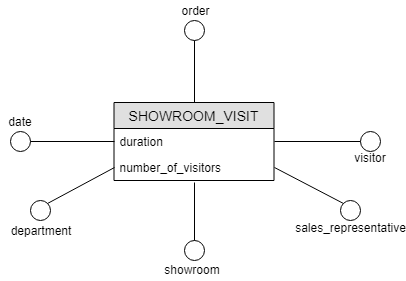
\includegraphics[scale=0.65]{../images/DFM_Showroom_Simple.png}
        \caption{
                \label{fig:showroom}  
                DFM of the showroom visit
        }
\end{figure}

\begin{figure}[H] 
        \centering
        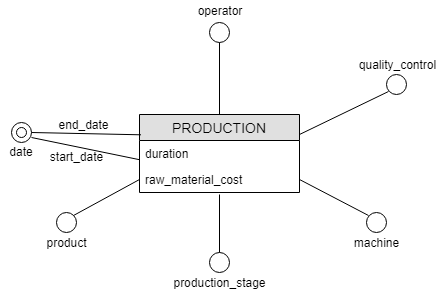
\includegraphics[scale=0.65]{../images/DFM_Production_Simple.png}
        \caption{
                \label{fig:production}  
                DFM of the production
        }
\end{figure}

\subsection{Showroom visit}

\begingroup
\renewcommand\arraystretch{0.5}
\begin{longtable}{p{3.7cm}p{10cm}}
        \caption{Fact table Showroom} \\
        Dimension & Attributes \\
        \endfirsthead \\
        Dimension & Attributes \\
        \endhead \\
        \hline \\
        Date & Day, Month, Year, Quartal, Week, Day of Week, Season, Holiday \\
        \hline \\
        Showroom & Name, City, District, Province, Region, Country, Manager, Address, Telephone, Size \\
        \hline \\
        Visitor & Name, City, District, Province, Region, Country, Language, Telephone, E-Mail, Type, Sector, Gender, Customer number \\
        \hline \\
        Order & Order Number, Total Price, Discount \\
        \hline \\
        Order Detail & Quantity, Quantity Type, Product, Unit price, Total price \\
        \hline \\
        Department & Name \\
        \hline \\
        Sales representative & Name, City, District, Province, Region, Country, Language, Telephone, E-Mail, Gender \\
        \hline \\
\end{longtable}
\endgroup

\begin{figure}[H] 
        \centering
        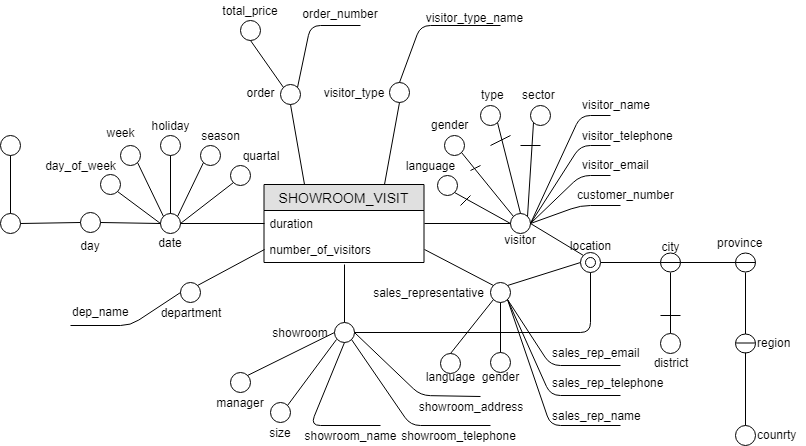
\includegraphics[width=\columnwidth]{../images/DFM_Showroom.png}
        \caption{
                \label{fig:showroomAttributes}  
                Dimension fact model (DFM) of the showroom visit with attributes 
        }
\end{figure}

\subsection{Production}

\begingroup
\renewcommand\arraystretch{0.5}
\begin{longtable}{p{4cm}p{9cm}}
        \caption{Fact table Production} \\
        Dimension & Attributes \\
        \endfirsthead \\
        Dimension & Attributes \\
        \endhead \\
        \hline \\
        Start date & Day, Month, Year, Week \\
        \hline \\
        End date & Day, Month, Year, Week \\
        \hline \\
        Product & Product number, Name, Department, Category \\
        \hline \\
        Production stage & Name \\
        \hline \\
        Machine & Name, Purchasing year, Vendor \\
        \hline \\
        Quality control & Grade \\
        \hline \\
        Operator & Name \\
        \hline \\
\end{longtable}
\endgroup

\begin{figure}[h] 
        \centering
        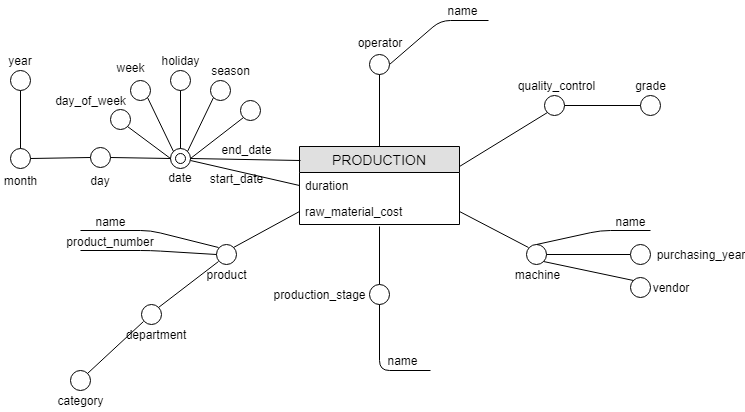
\includegraphics[width=\columnwidth]{../images/DFM_Production.png}
        \caption{
                \label{fig:productionAttributes}  
                Dimension fact model (DFM) of the production with attributes 
        }
\end{figure}

\section{Logical Design}

\subsection{Star schemas}

The following star schema fig. \ref{fig:starschemaShowroom} represent the first business process, namely the showroom visit. In order for being able to obtain more detailed query results, we decided to create the foreign table 'location'. With this approach for example, we are able to understand, from which particular place are the different visitors coming and are visiting which showroom in which location. Also for marketing decision the location of the showroom and the location of the different visitors is crucial.

\begin{figure}[H] 
        \centering
        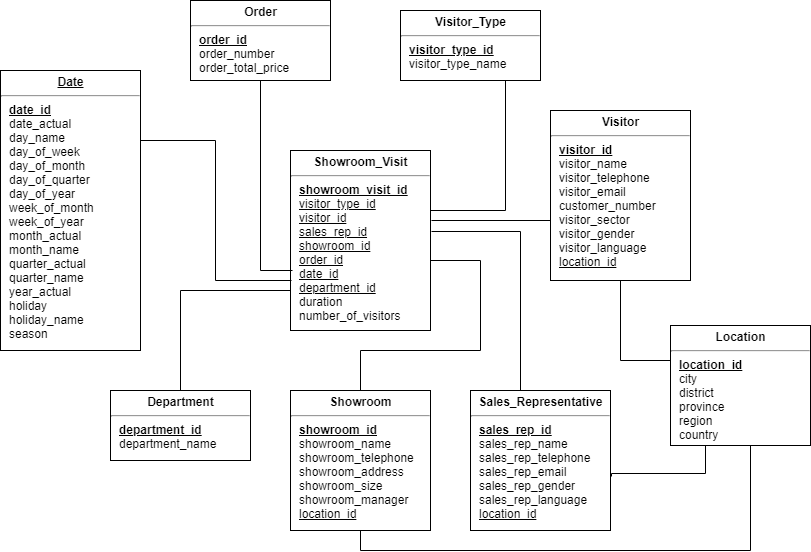
\includegraphics[width=\columnwidth]{../images/Starschema_Showroom_visit.png}
        \caption{
                \label{fig:starschemaShowroom}  
                Star schema of the showroom visit
        }
\end{figure}

Instead, the star schema fig. \ref{fig:starschemaProduction} represents the production business process.

\begin{figure}[H] 
        \centering
        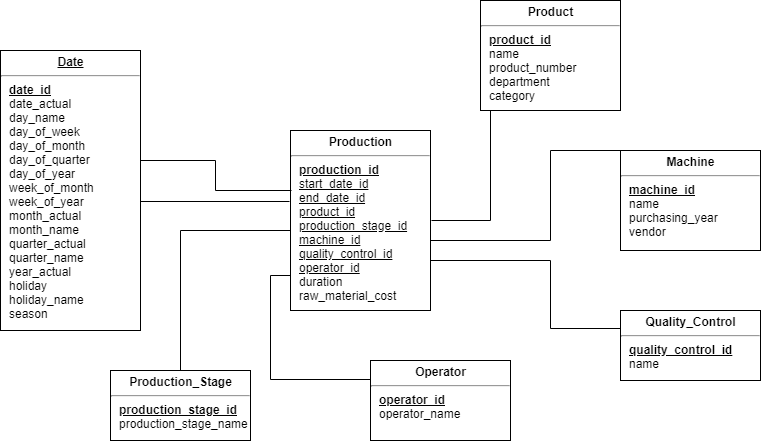
\includegraphics[width=\columnwidth]{../images/Starschema_Production.png}
        \caption{
                \label{fig:starschemaProduction}  
                Star schema of the production
        }
\end{figure}

\subsection{Two business questions}

\subsubsection{Fact: Showroom visit}

In order to be able to make the right marketing decisions, it is very important for the management to know from which sector the various customers or interested parties of a particular showroom come from. So, for example the management wants to know, from which sectors the various customers of showroom "Showroom-Bozen" were coming in the last year.

\bigskip
\noindent SQL query:
\begin{lstlisting}[
        language=SQL,
        showspaces=false,
        basicstyle=\ttfamily,
        numbers=left,
        numberstyle=\tiny,
        commentstyle=\color{gray}
     ]
SELECT v.visitor_sector, count(*)
FROM warehouse.visitor v
INNER JOIN warehouse.showroom_visit sv on v.visitor_id = sv.visitor_id
INNER JOIN warehouse.showroom s on sv.showroom_id = s.showroom_id
INNER JOIN warehouse.date d on sv.date_id = d.date_id
WHERE s.showroom_name = 'Showroom-BOZEN' 
AND d.date_actual >= '2018-01-01' AND d.date_actual <= '2018-12-31'
GROUP by v.visitor_sector
\end{lstlisting}

\begingroup
\renewcommand\arraystretch{0.5}
\begin{longtable}{p{1.4cm}p{1.5cm}p{1.8cm}p{1.5cm}p{1.6cm}p{1.4cm}p{1.2cm}p{1.25cm}p{1.85cm}}
        \caption{Showroom visit} \\
        ID & Visitor\_id & Sales\_rep\_id & Showr.\_id & Depart.\_id & Date\_id & Type\_id & Duration & Nr.\_of\_visit. \\
        \endfirsthead \\
        ID & Visitor\_id & Sales\_rep\_id & Showr.\_id & Depart.\_id & Date\_id & Type\_id & Duration & Nr.\_of\_visit. \\
        \endhead \\
        \hline \\
        1282369	& \color{red} 570822 & 6 & \color{red} 5 & 4 & \color{red}20180323 & 2 & 90 & 2 \\
        \hline \\
        1282370	& 570823 & 5 & 5 & 2 & 20160107 & 4 & 167 & 4 \\
        \hline \\
        1282371	& 570823 & 7 & 5 & 1 & 20130526 & 3 & 173 & 6 \\
        \hline \\
        1282372	& 570823 & 11 & 5 & 6 & 20150806  & 3 & 100 & 10 \\
        \hline \\
        1282373	& 570823 & 7 & 5 & 1 & 20121116 & 4 & 169 & 5 \\
        \hline \\
        1282374	& 570824 & 7 & 5 & 1 & 20171210 & 3 & 57 & 3 \\
        \hline \\
        1282375	& 570824 & 18 & 5 & 2 & 20110212 & 3 & 166 & 7 \\
        \hline \\
        1282376	& 570824 & 9 & 5 & 4 & 20130811  & 3 & 84 & 5 \\
        \hline \\
        1282377	& 570825 & 11 & 5 & 6 & 20170507 & 3 & 184 & 10 \\
        \hline \\
        1282378	& 570825 & 12 & 5 & 2 & 20111127 & 2 & 26 & 2 \\
        \hline \\
        1282379	& 570825 & 7 & 5 & 1 & 20150425 & 3 & 141 & 10 \\
        \hline \\
        1282380	& 570826 & 11 & 5 & 6 & 20130208 & 2 & 8 & 2 \\
        \hline \\
        1282381	& 570826 & 12 & 5 & 1 & 20111214 & 3 & 61 & 8 \\
        \hline \\
        1282382	& 570827 & 12 & 5 & 1 & 20170202 & 3 & 139 & 9 \\
        \hline \\
        1282383 & 570827 & 12 & 5 & 2 & 20121012 & 3 & 71 & 7 \\
        \hline \\
\end{longtable}
\endgroup

\begingroup
\renewcommand\arraystretch{0.5}
\begin{longtable}{p{1.3cm}p{1.6cm}p{1.8cm}p{3.6cm}p{2cm}p{.7cm}p{1.2cm}p{1.4cm}}
        \caption{Visitor} \\
        ID & Name & Telephone & E-Mail & Sector & Sex & Lang. & Loc.\_id \\
        \endfirsthead \\
        ID & Name & Telephone & E-Mail & Sector & Sex & Lang. & Loc.\_id \\
        \endhead \\
        \hline \\
        \color{red} 570822 & Melanie Eder &  &  & \color{red} Gastronomy & F & german & 9 \\
        \hline \\
        570823 & Julian Schmidt &  & j.schmidt@email.com & \color{red} Private & M & german & 9 \\
        \hline \\
        570824 & Marcel Schwarz & 306 9579783 & m.schwarz@email.com & \color{red} Hotel & M & german & 9 \\
        \hline \\
        570825 & Denise Fuchs & 396 5305260 & d.fuchs@email.com & \color{red} Public & F & german & 9 \\
        \hline \\
        570826 & Sophie Wimmer & 322 7641804 & s.wimmer@email.com & \color{red} Private & F & german & 9 \\
        \hline \\
\end{longtable} 
\endgroup

\begingroup
\renewcommand\arraystretch{0.5}
\begin{longtable}{p{0.25cm}p{3.9cm}p{2.2cm}p{2.9cm}p{.7cm}p{3.1cm}p{1.1cm}}
        \caption{Showroom} \\
        ID & Name & Telephone & Address & Size & Manager & Loc.\_id \\
        \endfirsthead \\
        ID & Name & Telephone & Address & Size & Manager & Loc.\_id \\
        \endhead \\
        \hline \\
        1 & Showroom-LATSCH & 0477 069655 & Herrengasse 8 & 581 & Paul Wolf & 42 \\
        \hline \\
        2 & Showroom-M{\"U}HLBACH & 0474 039227 & Platzerstr. 58 & 349 & Christoph Steiner & 54 \\
        \hline \\
        3 & Showroom-M{\"O}LTEN & 0470 429676 & Vernag 97 & 857 & Christoph Steiner & 51 \\
        \hline \\
        4 & Showroom-SALURN & 0475 248487 & Gewerbezone 44 & 198 & Johannes Egger & 77 \\
        \hline \\
        \color{red} 5 & \color{red} Showroom-BOZEN & 0473 723301 & St. Urban 73 & 447 & Sabine Schneider & 9 \\
        \hline \\
\end{longtable} 
\endgroup

\begingroup
\renewcommand\arraystretch{0.5}
\begin{longtable}{p{1.5cm}p{2cm}p{1.5cm}p{1.5cm}p{1.3cm}p{1.1cm}p{0.7cm}p{1.1cm}p{1.2cm}}
        \caption{Date} \\
        ID & Date & Day\_week & Day & Month & Quartal & Year & Holiday & Season \\
        \endfirsthead \\
        ID & Date & Day\_week & Day & Month & Quartal & Year & Holiday & Season \\
        \endhead \\
        \hline \\
        20160102 & 2010-01-02 & 6 & Saturday & January & First & 2016 & false & Winter \\
        \hline \\
        20170103 & 2010-01-03 & 7 & Sunday & January & First & 2017 & false & Winter \\
        \hline \\
        20180108 & \color{red} 2018-01-08 & 5 & Friday & January & First & 2018 & false & Winter \\
        \hline \\
        20190109 & 2010-01-09 & 6 & Saturday & January & First & 2019 & false & Winter \\
        \hline \\
        20200110 & 2010-01-10 & 7 & Sunday & January & First & 2020 & false & Winter \\
        \hline \\
\end{longtable} 
\endgroup

\begingroup
\renewcommand\arraystretch{0.5}
\begin{longtable}{p{3cm}p{4cm}}
        \caption{Result of the query} \\
        Sector & Number of visits \\
        \endfirsthead \\
        Sector & Number of visits \\
        \endhead \\
        \hline \\
        Gastronomy & 2985 \\
        \hline \\
        Hotel & 4223 \\
        \hline \\
        Private & 5629 \\
        \hline \\
        Public & 1371 \\
        \hline \\
\end{longtable} 
\endgroup

\subsubsection{Fact: Production}

The company's quality control is always interested in optimizing processes. It is therefore interesting for employees to know whether a machine has significant time differences in production in relation to a particular product in comparison to the other machines.

\bigskip
\noindent SQL query:
\begin{lstlisting}[
        language=SQL,
        showspaces=false,
        basicstyle=\ttfamily,
        numbers=left,
        numberstyle=\tiny,
        commentstyle=\color{gray}
     ]
SELECT m.machine_name, avg(p.duration) AS avg_production_duration
FROM warehouse.machine m
INNER JOIN warehouse.production p ON m.machine_id = p.machine_id
INNER JOIN warehouse.product o ON p.product_id = o.product_id
WHERE o.product_number = 'Warteraum-Couch - 10'
GROUP BY m.machine_id
ORDER BY avg_production_duration DESC LIMIT 10
\end{lstlisting}

\begingroup
\renewcommand\arraystretch{0.5}
\begin{longtable}{p{1cm}p{1.5cm}p{1.5cm}p{1cm}p{1.5cm}p{1.8cm}p{1.6cm}p{1.3cm}p{2.2cm}}
        \caption{Production} \\
        ID & Operator* & Machine* & Stage* & Product* & Start\_date* & End\_date* & Duration & Raw\_mat.\_cost \\
        \endfirsthead \\
        ID & Operator* & Machine* & Stage* & Product* & Start\_date* & End\_date* & Duration & Raw\_mat.\_cost \\
        \endhead \\
        \hline \\
        591814 & 779 & 1144 & 1 & \color{red} 361016 & 20101105 & 20101202 & \color{red} 152 & 76 \\
        \hline \\
        591815 & 780 & 1174 & 2 & \color{red} 361016 & 20101202 & 20101203 & \color{red} 1 & 395 \\
        \hline \\
        591816 & 775 & 1213 & 3 & \color{red} 361016 & 20101203 & 20101207 & \color{red} 2 & 277 \\
        \hline \\
        591817 & 770 & 1055 & 1 & \color{red} 361016 & 20101122 & 20101214 & \color{red} 30 & 66 \\
        \hline \\
        591818 & 722 & \color{red} 1176 & 2 & \color{red} 361016 & 20101214 & 20110111 & \color{red} 133 & 391 \\
        \hline \\
        591819 & 755 & 1079 & 3 & \color{red} 361016 & 20110111 & 20110204 & \color{red} 36 & 275 \\
        \hline \\
        591820 & 740 & 1069 & 1 & \color{red} 361016 & 20150511 & 20150520 & \color{red} 49 & 73 \\
        \hline \\
        591821 & 756 & 1025 & 2 & \color{red} 361016 & 20150520 & 20150603 & \color{red} 54 & 398 \\
        \hline \\
        591822 & 758 & 1130 & 3 & \color{red} 361016 & 20150603 & 20150625 & \color{red} 96 & 278 \\
        \hline \\
        27064 & 754 & 1164 & 1 & \color{red} 361016 & 20101022 & 20101026 & \color{red} 8 & 66 \\
        \hline \\
        27065 & 739 & 1028 & 2 & \color{red} 361016 & 20101026 & 20101104 & \color{red} 6 & 407 \\
        \hline \\
        27066 & 798 & 1098 & 3 & \color{red} 361016 & 20101104 & 20101105 & \color{red} 6 & 280 \\
        \hline \\
        27067 & 780 & 1013 & 1 & \color{red} 361016 & 20130327 & 20130411 & \color{red} 70 & 74 \\
        \hline \\
        27068 & 737 & 1145 & 2 & \color{red} 361016 & 20130411 & 20130509 & \color{red} 18 & 404 \\
        \hline \\
        27069 & 772 & 1032 & 3 & \color{red} 361016 & 20130509 & 20130520 & \color{red} 14 & 281 \\
        \hline \\
\end{longtable} 
\endgroup

Note: all columns with the * are foreign key columns and are carrying only the id

\begingroup
\renewcommand\arraystretch{0.5}
\begin{longtable}{p{1cm}p{3cm}p{3.2cm}p{3.1cm}}
        \caption{Machine} \\
        ID & Machine\_name & Machine\_vendor & Purchasing\_year \\
        \endfirsthead \\
        ID & Machine\_name & Machine\_vendor & Purchasing\_year \\
        \endhead \\
        \hline \\
        1172 & Melichár & Durán & 1998 \\
        \hline \\
        1173 & Horn & Lóntos & 2009 \\
        \hline \\
        1174 & Chihaia & Murtazaev & 2002 \\
        \hline \\
        1175 & Korčák & Durán & 2006 \\
        \hline \\
        \color{red} 1176 & \color{red} Ramóna & Barbora & 1996 \\
        \hline \\
\end{longtable} 
\endgroup

\begingroup
\renewcommand\arraystretch{0.5}
\begin{longtable}{p{1.4cm}p{2.7cm}p{3.7cm}p{3.4cm}p{3cm}}
        \caption{Product} \\
        ID & Product\_name & Product\_number & Product\_department & Product\_category \\
        \endfirsthead \\
        ID & Product\_name & Product\_number & Product\_department & Product\_category \\
        \endhead \\
        \hline \\
        361013 & Warteraum-Couch & Warteraum-Couch - 7 & Büro & Arztpraxis-Set \\
        \hline \\
        361014 & Warteraum-Couch & Warteraum-Couch - 8 & Büro & Arztpraxis-Set \\
        \hline \\
        361015 & Warteraum-Couch & Warteraum-Couch - 9 & Büro & Arztpraxis-Set \\
        \hline \\
        \color{red} 361016 & Warteraum-Couch & \color{red} Warteraum-Couch - 10 & Büro & Arztpraxis-Set \\
        \hline \\
        361017 & Warteraum-Couch & Warteraum-Couch - 11 & Büro & Arztpraxis-Set \\
        \hline \\
\end{longtable} 
\endgroup

\begingroup
\renewcommand\arraystretch{0.5}
\begin{longtable}{p{3cm}p{4cm}}
        \caption{Result of the query} \\
        Machine\_name & AVG\_Production\_duration \\
        \endfirsthead \\
        Machine\_name & AVG\_Production\_duration \\
        \endhead \\
        \hline \\
        Vajda & 152.00 \\
        \hline \\
        \color{red} Ramóna & 133.00 \\
        \hline \\
        Papandreou & 96.00 \\
        \hline \\
        Kontoléon & 70.00 \\
        \hline \\
        Mitu & 54.00 \\
        \hline \\
        Bercu & 49.00 \\
        \hline \\
        Heinrich & 36.00 \\
        \hline \\
        Martinez & 30.00 \\
        \hline \\
        Pál & 18.00 \\
        \hline \\
        Aguilar & 14.00 \\
        \hline \\
\end{longtable} 
\endgroup

\section{Implementation}


\subsection{Creation}

\subsubsection{Showroom data mart}
This sql script creates the table structure for the showroom visit data mart:

\begin{lstlisting}[
        language=SQL,
        showspaces=false,
        basicstyle=\ttfamily,
        numbers=left,
        numberstyle=\tiny,
        commentstyle=\color{gray}
     ]
CREATE TABLE IF NOT EXISTS warehouse.location(
  	location_id SERIAL PRIMARY KEY NOT NULL,
  	city VARCHAR(100) NULL,
  	district VARCHAR(100) NULL,
	province VARCHAR(100) NULL,
	region VARCHAR(100) NULL,
	country VARCHAR(100) NOT NULL
);

CREATE TABLE IF NOT EXISTS warehouse.date
(
       date_id SERIAL PRIMARY KEY NOT NULL,
       date_actual DATE NOT NULL,
       day_name VARCHAR(9) NOT NULL,
       day_of_week INT NOT NULL,
       day_of_month INT NOT NULL,
       day_of_quarter INT NOT NULL,
       day_of_year INT NOT NULL,
       week_of_month INT NOT NULL,
       week_of_year INT NOT NULL,
       month_actual INT NOT NULL,
       month_name VARCHAR(9) NOT NULL,
       quarter_actual INT NOT NULL,
       quarter_name VARCHAR(9) NOT NULL,
       year_actual INT NOT NULL,
       mmyyyy CHAR(6) NOT NULL,
       mmddyyyy CHAR(10) NOT NULL,
       holiday BOOLEAN NOT NULL,
       holiday_name VARCHAR(50),
       season VARCHAR(20)
);

CREATE INDEX d_date_date_actual_idx ON warehouse.date(date_actual);

CREATE TABLE IF NOT EXISTS warehouse.visitor(
	visitor_id SERIAL PRIMARY KEY NOT NULL,
	visitor_name VARCHAR(100),
	visitor_telephone VARCHAR(100),
	visitor_email VARCHAR(100),
	customer_number VARCHAR(100),
	visitor_sector VARCHAR(50),
	visitor_gender VARCHAR(10),
	visitor_language VARCHAR(50),
	visitor_location_id int REFERENCES 
		warehouse.location(location_id)
);


CREATE TABLE IF NOT EXISTS warehouse.sales_representative(
	sales_rep_id SERIAL PRIMARY KEY NOT NULL,
	sales_rep_name VARCHAR(100) NOT NULL,
	sales_rep_telephone VARCHAR(100) NOT NULL,
	sales_rep_email VARCHAR(100) NOT NULL,
	sales_rep_gender VARCHAR(10) NOT NULL,
	sales_rep_language VARCHAR(50) NOT NULL,
	sales_rep_location_id int REFERENCES 
		warehouse.location(location_id) NOT NULL
);


CREATE TABLE IF NOT EXISTS warehouse.showroom(
	showroom_id SERIAL PRIMARY KEY NOT NULL,
	showroom_name VARCHAR(100) NOT NULL,
	showroom_telephone VARCHAR(100) NOT NULL,
	showroom_address VARCHAR(100) NOT NULL,
	showroom_size int NOT NULL,
	showroom_manager VARCHAR(100) NOT NULL,
	showroom_location_id int REFERENCES 
		warehouse.location(location_id) NOT NULL
);


CREATE TABLE IF NOT EXISTS warehouse.department(
	department_id SERIAL PRIMARY KEY NOT NULL,
	department_name VARCHAR(100) NOT NULL
);

CREATE TABLE IF NOT EXISTS warehouse.order(
	order_id SERIAL PRIMARY KEY NOT NULL,
	order_number VARCHAR(100) NOT NULL,
	order_total_price numeric NOT NULL
);


CREATE TABLE IF NOT EXISTS warehouse.visitor_type(
	visitor_type_id SERIAL PRIMARY KEY NOT NULL,
	visitor_type_name VARCHAR(100) NOT NULL
);

CREATE TABLE IF NOT EXISTS warehouse.showroom_visit(
	showroom_visit_id SERIAL PRIMARY KEY NOT NULL,
	visitor_id int REFERENCES warehouse.visitor(visitor_id),
	sales_rep_id int REFERENCES 
		warehouse.sales_representative(sales_rep_id) NOT NULL,
	showroom_id int REFERENCES 
		warehouse.showroom(showroom_id) NOT NULL,
	department_id int REFERENCES 
		warehouse.department(department_id) NOT NULL,
	date_id int REFERENCES warehouse.date(date_id) NOT NULL,
	order_id int REFERENCES warehouse.order(order_id),
	visitor_type_id int REFERENCES 
		warehouse.visitor_type(visitor_type_id),
	duration int NOT NULL,
	number_of_visitors int NOT NULL
);

\end{lstlisting}


\subsubsection{Production data mart}
Whereas, this script creates the needed tables for the production data mart:

\begin{lstlisting}[
        language=SQL,
        showspaces=false,
        basicstyle=\ttfamily,
        numbers=left,
        numberstyle=\tiny,
        commentstyle=\color{gray}
     ]
		
CREATE TABLE IF NOT EXISTS warehouse.operator(
  	operator_id SERIAL PRIMARY KEY NOT NULL,
  	operator_name VARCHAR(100) NOT NULL
);

CREATE TABLE IF NOT EXISTS warehouse.quality_control(
  	quality_control_id SERIAL PRIMARY KEY NOT NULL,
  	quality_control_grade int NOT NULL
);

CREATE TABLE IF NOT EXISTS warehouse.machine(
  	machine_id SERIAL PRIMARY KEY NOT NULL,
  	machine_name VARCHAR(100) NOT NULL,
  	machine_vendor VARCHAR(100) NOT NULL,
  	machine_purchasing_year int NOT NULL
);

CREATE TABLE IF NOT EXISTS warehouse.production_stage(
  	production_stage_id SERIAL PRIMARY KEY NOT NULL,
  	production_stage_name VARCHAR(100) NOT NULL
);

CREATE TABLE IF NOT EXISTS warehouse.product(
  	product_id SERIAL PRIMARY KEY NOT NULL,
  	product_name VARCHAR(100) NOT NULL,
  	product_number VARCHAR(100) NOT NULL,
  	product_department VARCHAR(100) NOT NULL,
  	product_category VARCHAR(100) NOT NULL
);

CREATE TABLE IF NOT EXISTS warehouse.production(
	production_id SERIAL PRIMARY KEY NOT NULL,
	operator_id int REFERENCES 
		warehouse.operator(operator_id) NOT NULL,
	quality_control_id int REFERENCES 
		warehouse.quality_control(quality_control_id),
	machine_id int REFERENCES warehouse.machine(machine_id) NOT NULL,
	production_stage_id int REFERENCES 
		warehouse.production_stage(production_stage_id) NOT NULL,
	product_id int REFERENCES warehouse.product(product_id),
	start_date_id int REFERENCES warehouse.date(date_id) NOT NULL,
	end_date_id int REFERENCES warehouse.date(date_id) NOT NULL,
	duration int NOT NULL,
	raw_material_cost int NOT NULL
);		
		
\end{lstlisting}

\subsection{ROLLUP}
\subsubsection{SQL query using ROLLUP for business process 1 (showroom visit)}

The following sql query shows the number of visits per showroom, in the different areas and in the different seasons. In addition there are the different partial sums. For example, for the showroom in Bolzano, first the number of visits for the 'bedroom' area in autumn is shown, then the total number of visits for the 'bedroom' area, regardless of the season, and finally the total number of visits for the showroom in Bolzano, regardless of the area and the season.

\begin{lstlisting}[
        language=SQL,
        showspaces=false,
        basicstyle=\ttfamily,
        numbers=left,
        numberstyle=\tiny,
        commentstyle=\color{gray}
     ]
SELECT showroom_name, department_name, season, count(visitor_id)
FROM warehouse.showroom_visit
JOIN warehouse.showroom using (showroom_id)
JOIN warehouse.department using (department_id)
JOIN warehouse.date using (date_id)
GROUP BY ROLLUP(showroom_name, department_name, season);
\end{lstlisting}


\begingroup
\renewcommand\arraystretch{0.5}
\begin{longtable}{p{4cm}p{4cm}p{3cm}p{2cm}}
        \caption{Showroom ROLLUP Result} \\
	showroom\_name & department\_name & season & count \\
        \endfirsthead \\
        showroom\_name & department\_name & season & count \\
        \endhead \\
        \hline \\
	Showroom-BOZEN & Badezimmer & Frühling & 2579 \\
        \hline \\
        Showroom-BOZEN & Badezimmer & Herbst & 3285 \\
        \hline \\
        Showroom-BOZEN & Badezimmer & Sommer & 1311 \\
        \hline \\
        Showroom-BOZEN & Badezimmer & Winter & 4708 \\
        \hline \\
        Showroom-BOZEN & Badezimmer & * & 11883 \\
        \hline \\
        Showroom-BOZEN & Büro & Frühling & 298 \\
        \hline \\
        Showroom-BOZEN & Büro & Herbst & 281 \\
        \hline \\
        Showroom-BOZEN & Büro & Sommer & 156 \\
        \hline \\
        Showroom-BOZEN & Büro & Winter & 480 \\
        \hline \\
        Showroom-BOZEN & Büro & * & 1215 \\
        \hline \\
        Showroom-BOZEN & Hotel & Frühling & 4032 \\
        \hline \\
        Showroom-BOZEN & Hotel & Herbst & 4472 \\
        \hline \\
        Showroom-BOZEN & Hotel & Sommer & 2022 \\
        \hline \\
        Showroom-BOZEN & Hotel & Winter & 6808 \\
        \hline \\
        Showroom-BOZEN & Hotel & * & 17334 \\
        \hline \\
        ... \\
        \hline \\
\end{longtable} 
\endgroup

\subsubsection{SQL query with ROLLUP for business process 2 (production)}

The following sql query shows the average machining time for a particular production stage of a particular product of a particular product category. The query also returns the average machining times of the higher levels, in other words, a granularity is removed step by step. For example, the average machining time of 'table XY' is shown first for the 'fine grinding' process. Then you get the average machining time of all processes on 'table XY' and finally the average machining time of all processes on all table models, thus of the whole product category 'table'.

\begin{lstlisting}[
        language=SQL,
        showspaces=false,
        basicstyle=\ttfamily,
        numbers=left,
        numberstyle=\tiny,
        commentstyle=\color{gray}
     ]
SELECT product_category, product_name, 
        production_stage_name, ROUND(avg(duration)::numeric,2) as avg
FROM warehouse.production
JOIN warehouse.product using (product_id)
JOIN warehouse.production_stage using (production_stage_id)
GROUP BY ROLLUP(product_category, product_name, production_stage_name);
\end{lstlisting}    


\begingroup
\renewcommand\arraystretch{0.5}
\begin{longtable}{p{4cm}p{4cm}p{4cm}p{2cm}}
        \caption{Production ROLLUP Result} \\
	product\_category & product\_name & production\_stage\_name & avg \\
        \endfirsthead \\
        product\_category & product\_name & production\_stage\_name & avg \\
        \endhead \\
        \hline \\
        AdsH-Set & AdsH-Fähnchen & Ausführung & 44.28 \\
        \hline \\
        AdsH-Set & AdsH-Fähnchen & Feinschliff & 44.18 \\
        \hline \\
        AdsH-Set & AdsH-Fähnchen & Vorbereitung & 43.35 \\
        \hline \\
        AdsH-Set & AdsH-Fähnchen & * & 43.94 \\
        \hline \\
        AdsH-Set & AdsH-Goldabzeichen & Ausführung & 45.11 \\
        \hline \\
        AdsH-Set & AdsH-Goldabzeichen & Feinschliff & 44.15 \\
        \hline \\
        AdsH-Set & AdsH-Goldabzeichen & Vorbereitung & 43.71 \\
        \hline \\
        AdsH-Set & AdsH-Goldabzeichen & * & 44.32 \\
        \hline \\
        AdsH-Set & AdsH-Goldpokal & Ausführung & 46.37 \\
        \hline \\
        AdsH-Set & AdsH-Goldpokal & Feinschliff & 43.60 \\
        \hline \\
        AdsH-Set & AdsH-Goldpokal & Vorbereitung & 47.80 \\
        \hline \\
        ... \\
        \hline \\
\end{longtable} 
\endgroup

\subsection{CUBE}

\subsubsection{SQL query using CUBE for business process 1 (showroom visit)}

The following query shows the number of visitors from the province of Bolzano and its commercial sector in the different districts of the showrooms. In addition, the query shows all possible sub-totals, removing step by step different granularities. In other words, for each combination of values, the sum is shown, finally the total sum of all visits from visitors from the province of Bolzano.

\begin{lstlisting}[
        language=SQL,
        showspaces=false,
        basicstyle=\ttfamily,
        numbers=left,
        numberstyle=\tiny,
        commentstyle=\color{gray}
        ]
SELECT visitor_sector, vl.district as visitor_district, 
        sl.district as showroom_district, sum(number_of_visitors)
FROM warehouse.showroom_visit
JOIN warehouse.visitor using (visitor_id)
JOIN warehouse.location as vl 
        on warehouse.visitor.location_id = vl.location_id 
JOIN warehouse.showroom using (showroom_id)
JOIN warehouse.location as sl 
        on warehouse.showroom.location_id = sl.location_id
WHERE vl.province = 'Bozen'
GROUP BY CUBE(vl.district, visitor_sector, sl.district)
ORDER BY visitor_sector, vl.district, sl.district;
\end{lstlisting}

\begingroup
\renewcommand\arraystretch{0.5}
\begin{longtable}{p{4cm}p{3cm}p{4cm}p{2cm}}
        \caption{Showroom CUBE Result} \\
	visitor\_sector & visitor\_district & showroom\_district & sum \\
        \endfirsthead \\
        visitor\_sector & visitor\_district & showroom\_district & sum \\
        \endhead \\
        \hline \\
        Gastronomy & Bozen & Bozen & 55749 \\
        \hline \\
        Gastronomy & Bozen & Burggrafenamt  & 2574 \\
        \hline \\
        Gastronomy & Bozen & Eisacktal & 1554 \\
        \hline \\
        Gastronomy & Bozen & Pustertal & 2887 \\
        \hline \\
        Gastronomy & Bozen & Salten Schlern & 3501 \\
        \hline \\
        Gastronomy & Bozen & Überetsch-Südtiroler Unterland & 1842 \\
        \hline \\
        Gastronomy & Bozen & Vinschgau & 2278 \\
        \hline \\
        Gastronomy & Bozen & Wipptal & 3031 \\
        \hline \\
        Gastronomy & Bozen & * & 73416 \\
        \hline \\
        ... \\
        \hline \\
\end{longtable} 
\endgroup

\subsubsection{SQL query using CUBE for business process 2 (production)}

The following query shows the average grade of the quality control for a machine and for the product category. Also all partial average values of all different combinations and groupings can be read off.

\begin{lstlisting}[
        language=SQL,
        showspaces=false,
        basicstyle=\ttfamily,
        numbers=left,
        numberstyle=\tiny,
        commentstyle=\color{gray}
     ]
SELECT product_department, machine_name, 
        ROUND(avg(quality_control_grade)::numeric,2) as avg
FROM warehouse.production
JOIN warehouse.product using (product_id)
JOIN warehouse.machine using (machine_id)
JOIN warehouse.quality_control using (quality_control_id)
WHERE quality_control_grade is not NULL
GROUP BY CUBE(product_department, machine_name)
ORDER BY product_department;	
\end{lstlisting}

\begingroup
\renewcommand\arraystretch{0.5}
\begin{longtable}{p{4cm}p{4.3cm}p{2cm}}
        \caption{Production CUBE Result} \\
	product\_department & machine\_name & avg \\
        \endfirsthead \\
        product\_department & machine\_name & avg \\
        \endhead \\
        \hline \\
        Badezimmer & José Alberto Córdova & 5.00 \\
        \hline \\
        Badezimmer & Herrera & 4.59 \\
        \hline \\
        Badezimmer & Dzurjanin & 4.46 \\
        \hline \\
        Badezimmer & Șchiopu & 4.44 \\
        \hline \\
        Badezimmer & Groșescu & 4.53 \\
        \hline \\
        Badezimmer & Văcăroiu & 4.46 \\
        \hline \\
        Badezimmer & Germanós & 4.47 \\
        \hline \\
        Badezimmer & Holuby & 4.42 \\
        \hline \\
        Badezimmer & Bogza & 4.31 \\
        \hline \\
        Badezimmer & Păcurariu & 4.34 \\
        \hline \\
        Badezimmer & Giurescu & 4.42 \\
        \hline \\
        Badezimmer & Raudsepp & 4.63 \\
        \hline \\
        Badezimmer & Argeșanu & 4.67 \\
        \hline \\
        Badezimmer & Ciupe & 4.14 \\
        \hline \\
        Badezimmer & Linda & 4.53 \\
        \hline \\
        ... \\
        \hline \\
\end{longtable} 
\endgroup  

\subsection{GROUPING SETS}

\subsubsection{SQL query using GROUPING SETS for business process 1 (showroom visit)}

The following query shows the sum of order prices per language served by a sales representative in a showroom. Also the total sum on order prices can be taken from a language in that showroom as well as the total sum served by that sales representative.

\begin{lstlisting}[
        language=SQL,
        showspaces=false,
        basicstyle=\ttfamily,
        numbers=left,
        numberstyle=\tiny,
        commentstyle=\color{gray}
        ]
SELECT showroom_name, sales_rep_name, 
        visitor_language, sum(order_total_price)
FROM warehouse.showroom_visit
JOIN warehouse.visitor using (visitor_id)
JOIN warehouse.sales_representative using (sales_rep_id)
JOIN warehouse.order using (order_id)
JOIN warehouse.showroom using (showroom_id)
GROUP BY GROUPING SETS(
        (showroom_name, sales_rep_name, visitor_language),
        (showroom_name, visitor_language),
        (showroom_name, sales_rep_name));
\end{lstlisting} 

\begingroup
\renewcommand\arraystretch{0.5}
\begin{longtable}{p{4cm}p{4cm}p{3cm}p{3cm}}
        \caption{Showroom CUBE Result} \\
	showroom\_name & sales\_rep\_name & visitor\_language & sum \\
        \endfirsthead \\
        showroom\_name & sales\_rep\_name & visitor\_language & sum \\
        \endhead \\
        \hline \\
        Showroom-BOZEN & Caroline Eder & english & 277049.23 \\
        \hline \\
        Showroom-BOZEN & Elisabeth Schwarz & english & 240820.64 \\
        \hline \\
        Showroom-BOZEN & Noemi Bruno & english & 8688.9 \\
        \hline \\
        Showroom-BOZEN & Simone Serra & english & 265751.20 \\
        \hline \\
        Showroom-BOZEN & Valerio Adami & english & 184714.18 \\
        \hline \\
        Showroom-BOZEN & * & english & 977024.15 \\
        \hline \\
        Showroom-BOZEN & Caroline Eder & german & 5384090.56 \\
        \hline \\
        Showroom-BOZEN & Elisabeth Schwarz & german & 8917292.85 \\
        \hline \\
        Showroom-BOZEN & Mario Lang & german & 2448919.46 \\
        \hline \\
        Showroom-BOZEN & Martina Lehner & german & 3255981.32 \\
        \hline \\
        Showroom-BOZEN & Noemi Bruno & german & 6188561.63 \\
        \hline \\
        Showroom-BOZEN & Simone Serra & german & 4546093.16 \\
        \hline \\
        Showroom-BOZEN & Valerio Adami & german & 5940355.45 \\
        \hline \\
        Showroom-BOZEN & * & german & 36681294.43 \\
        \hline \\
        ... \\
        \hline \\
\end{longtable} 
\endgroup           

\subsubsection{SQL query using GROUPING SETS for business process 2 (production)}

The following query shows the number of a certain grade for a product category in a specific year. The query also shows the number of a certain rating in a certain year.

\begin{lstlisting}[
        language=SQL,
        showspaces=false,
        basicstyle=\ttfamily,
        numbers=left,
        numberstyle=\tiny,
        commentstyle=\color{gray}
        ]
SELECT product_category, year_actual, 
        quality_control_grade, count(product_id)
FROM warehouse.production
JOIN warehouse.product using (product_id)
JOIN warehouse.date ON date.date_id = production.end_date_id
JOIN warehouse.quality_control using (quality_control_id)
GROUP BY GROUPING SETS(
        (product_category, year_actual, quality_control_grade),
        (year_actual, quality_control_grade));
\end{lstlisting}

\begingroup
\renewcommand\arraystretch{0.5}
\begin{longtable}{p{4cm}p{3cm}p{4cm}p{2cm}}
        \caption{Production GROUPING SETS Result} \\
	product\_category & year\_actual & quality\_control\_grade & count
        \endfirsthead \\
        product\_category & year\_actual & quality\_control\_grade & count
        \endhead \\
	\hline \\
        AdsH-Set & 2010 & 0 & 2 \\
        \hline \\
        Arztpraxis-Set & 2010 & 0 & 32 \\
        \hline \\
        Bonsai-Set & 2010 & 0 & 8 \\
        \hline \\
        Bühnen-Set & 2010 & 0 & 11 \\
        \hline \\
        Café-Set & 2010 & 0 & 9 \\
        \hline \\
        Computer-Set & 2010 & 0 & 2 \\
        \hline \\
        Einsame-Insel-Set & 2010 & 0 & 8 \\
        \hline \\
        Forschung-Set & 2010 & 0 & 3 \\
        \hline \\
        Haushaltsgeräte-Set & 2010 & 0 & 4 \\
        \hline \\
        Heizgeräte-Set & 2010 & 0 & 9 \\
        \hline \\
        Küchen-Set & 2010 & 0 & 16 \\
        \hline \\
        Lampen-Set & 2010 & 0 & 7 \\
        \hline \\
        Masken-Set & 2010 & 0 & 2 \\
        \hline \\				
        ... & & & \\
        \hline \\
\end{longtable} 
\endgroup  

\section{Querying}

\subsection{NTILE}

\subsubsection{SQL query using NTILE for business process 1 (showroom visit)}

The following sql statement calculates the number of visits coming from a particular location of the province of Bolzano and assigns each row to a group from 1-4, depending on the size of the number of visits.

\begin{lstlisting}[
        language=SQL,
        showspaces=false,
        basicstyle=\ttfamily,
        numbers=left,
        numberstyle=\tiny,
        commentstyle=\color{gray}
        ]	 
SELECT vl.city, count(visitor_id), 
        NTILE(4) OVER (ORDER BY count(visitor_id)) AS TILE4
FROM warehouse.showroom_visit
JOIN warehouse.visitor using (visitor_id)
JOIN warehouse.location as vl 
        on warehouse.visitor.location_id = vl.location_id 
WHERE vl.province = 'Bozen'
GROUP BY vl.city;
\end{lstlisting}

\begingroup
\renewcommand\arraystretch{0.5}
\begin{longtable}{p{4cm}p{4cm}p{4cm}}
        \caption{Showroom NTILE Result} \\
	city & count & tile4 \\
        \endfirsthead \\
        city & count & tile4 \\
        \endhead \\
	\hline \\
        VINTL & 1116 & 1 \\
        \hline \\
        TOBLACH & 1149 & 1 \\
        \hline \\
        TERENTEN & 1161 & 1 \\
        \hline \\
        PRETTAU & 1166 & 1 \\
        \hline \\
        ENNEBERG & 1172 & 1 \\
        \hline \\
        GSIES & 1177 & 1 \\
        \hline \\
        ABTEI & 1195 & 1 \\
        \hline \\
        BRUNECK & 1221 & 1 \\
        \hline \\
        SEXTEN & 1235 & 1 \\
        \hline \\
        MÜHLWALD & 1235 & 1 \\
        \hline \\
        OLANG & 1241 & 1 \\
        \hline \\
        GAIS & 1250 & 1 \\
        \hline \\
        CORVARA & 1254 & 1 \\
        \hline \\
        ... & & \\
        \hline \\
\end{longtable} 
\endgroup
      
\subsubsection{SQL query using NTILE for business process 2 (production)}

The next sql query averages all processing times of an operator and groups them to 4 groups, were each operators gets assigned to a specific group relatively to the average of duration of all production steps.

\begin{lstlisting}[
        language=SQL,
        showspaces=false,
        basicstyle=\ttfamily,
        numbers=left,
        numberstyle=\tiny,
        commentstyle=\color{gray}
        ]
SELECT operator_name, ROUND(avg(duration)::numeric,2) as avg, 
	NTILE(4) OVER (ORDER BY avg(duration)) AS TILE4
	FROM warehouse.production
	JOIN warehouse.operator using (operator_id)
	GROUP BY operator_name;
\end{lstlisting}

\begingroup
\renewcommand\arraystretch{0.5}
\begin{longtable}{p{4cm}p{4cm}p{4cm}}
        \caption{Production NTILE Result} \\
	operator\_name & avg & tile4 \\
        \endfirsthead \\
        operator\_name & avg & tile4 \\
        \endhead \\
	\hline \\
        Machaela Moser & 43.51 & 1 \\
        \hline \\
        Clemens Bauer & 44.01 & 1 \\
        \hline \\
        Patrick Haas & 44.19 & 1 \\
        \hline \\
        Machaela Schmid & 44.20 & 1 \\
        \hline \\
        Alexander Wallner & 44.25 & 1 \\
        \hline \\
        Martina Wagner & 44.33 & 1 \\
        \hline \\
        Georg Steiner & 44.40 & 1 \\
        \hline \\
        Tanja Lehner & 44.43 & 1 \\
        \hline \\
        Johanna Maier & 44.51 & 1 \\
        \hline \\
        Viktoria Schmidt & 44.52 & 1 \\
        \hline \\
        Maximilian Schmid & 44.56 & 1 \\
        \hline \\
        ... & & \\
        \hline \\
\end{longtable} 
\endgroup


\subsection{RANK}

\subsubsection{SQL query using RANK for business process 1 (showroom visit)}

The following query identifies the overall total number of visits per showroom and ranks them according to their number of visits.

\begin{lstlisting}[
        language=SQL,
        showspaces=false,
        basicstyle=\ttfamily,
        numbers=left,
        numberstyle=\tiny,
        commentstyle=\color{gray}
        ]
SELECT showroom_name, count(distinct visitor_id), 
        RANK() OVER (ORDER BY count(distinct visitor_id) DESC)
FROM warehouse.showroom_visit
JOIN warehouse.showroom using (showroom_id)
GROUP BY showroom_name;
\end{lstlisting}

\begingroup
\renewcommand\arraystretch{0.5}
\begin{longtable}{p{4cm}p{4cm}p{3cm}}
        \caption{Showroom RANK Result} \\
	Showroom & Count & Rank \\
        \endfirsthead \\
        Showroom & Count & Rank \\
        \endhead \\
	\hline \\
        Showroom-BOZEN & 43863 & 1 \\
        \hline \\
        Showroom-ULTEN & 20032 & 2 \\
        \hline \\
        Showroom-SEXTEN & 18765 & 3 \\ 
        \hline \\
        Showroom-MÖLTEN & 18711 & 4 \\
        \hline \\
        Showroom-LATSCH & 18078 & 5 \\
        \hline \\
        Showroom-MÜHLBACH & 15183 & 6 \\ 
        \hline \\
        Showroom-SALURN & 14788 & 7 \\
        \hline \\
        Showroom-RATSCHINGS & 13442 & 8 \\ 
        \hline \\
        ... & & \\
        \hline \\
\end{longtable} 
\endgroup

\subsubsection{SQL query using RANK for business process 2 (production)}

The following sql query ranks the different products with respect to their average raw material costs.

\begin{lstlisting}[
        language=SQL,
        showspaces=false,
        basicstyle=\ttfamily,
        numbers=left,
        numberstyle=\tiny,
        commentstyle=\color{gray}
        ]
SELECT product_category, ROUND(avg(raw_material_cost)::numeric,2),
        RANK() OVER (ORDER BY (avg(raw_material_cost)) DESC)
FROM warehouse.production
JOIN warehouse.product using (product_id)
GROUP BY product_category;
\end{lstlisting}

\begingroup
\renewcommand\arraystretch{0.5}
\begin{longtable}{p{5cm}p{5cm}p{2cm}}
        \caption{Showroom RANK Result} \\
	Product\_category & AVG\_raw\_material\_cost & Rank \\
        \endfirsthead \\
        Product\_category & AVG\_raw\_material\_cost & Rank \\
        \endhead \\
        \hline \\
        Himmelsphänomene-Set & 373.96 & 1 \\
        \hline \\
        Sekretär-Set & 357.47 & 2 \\
        \hline \\
        Pflanzendeko-Set & 345.56 & 3 \\
        \hline \\
        Urkunden-Set & 324.72 & 4 \\
        \hline \\
        Melonen-Set & 319.97 & 5 \\
        \hline \\
        Regal-Set & 317.39 & 6 \\
        \hline \\
        Zitrus-Set & 315.05 & 7 \\
        \hline \\
        Kisten-Set & 314.72 & 8 \\
        \hline \\
        Frosch-Set & 312.50 & 9 \\
        \hline \\
        Birnen-Set & 312.47 & 10 \\
        \hline \\
        ... & & \\
        \hline \\
\end{longtable} 
\endgroup

\subsection{WINDOWING Clause}

\subsubsection{SQL query using a WINDOWING clause for business process 1 (showroom visit)}

The following windows clause query shows the total sum of orders of a particular day. In addition, using the functionality of a window function, the average of the last 7 days is shown.

\begin{lstlisting}[
        language=SQL,
        showspaces=false,
        basicstyle=\ttfamily,
        numbers=left,
        numberstyle=\tiny,
        commentstyle=\color{gray}
        ]																			   
SELECT date_actual, this_day, average_last_7_days	
FROM (
        SELECT date_actual, year_actual, sum(order_total_price) 
                as this_day, 
		ROUND(AVG(SUM(order_total_price))
			OVER ( ORDER BY date_actual
			ROWS BETWEEN 7 PRECEDING
                        AND CURRENT ROW)::numeric,2) 
                                as average_last_7_days
	FROM warehouse.showroom_visit
	JOIN warehouse.date using (date_id)
	JOIN warehouse.order using (order_id)
	GROUP BY date_actual, year_actual
        ORDER BY date_actual) 
AS res where year_actual > 2017;
\end{lstlisting}				  

\begingroup
\renewcommand\arraystretch{0.5}
\begin{longtable}{p{4cm}p{4cm}p{4cm}}
        \caption{Showroom WINDOWING Result} \\
	Date\_actual & this\_day & average\_last\_7\_days \\
        \endfirsthead \\
        Date\_actual & this\_day & average\_last\_7\_days \\
        \endhead \\
        \hline \\
        2018-01-01 & 679797.25 & 255967.71 \\
        \hline \\
        2018-01-02 & 68135.18 & 229689.79 \\
        \hline \\
        2018-01-03 & 187257.15 & 243683.57 \\
        \hline \\
        2018-01-04 & 180453.50 & 248296.45 \\
        \hline \\
        2018-01-05 & 402369.89 & 282831.82 \\
        \hline \\
        2018-01-06 & 463596.47 & 301014.82 \\
        \hline \\
        2018-01-07 & 427284.56 & 321012.68 \\
        \hline \\
        2018-01-08 & 24863.57 & 304219.70 \\
        \hline \\
        2018-01-09 & 97464.25 & 231428.07 \\
        \hline \\
        2018-01-10 & 5871.16" & 223645.07 \\
        \hline \\
        ... & & \\
        \hline \\
\end{longtable}
\endgroup

\subsubsection{SQL query using a WINDOWING clause for business process 2 (production)}

The following query sums the raw material costs of each month in the production. In addition, the average costs of raw material per month are calculated for the preceding six months.

\begin{lstlisting}[
        language=SQL,
        showspaces=false,
        basicstyle=\ttfamily,
        numbers=left,
        numberstyle=\tiny,
        commentstyle=\color{gray}
        ]			  
SELECT year_actual, month_actual, this_month, average_last_months
FROM (
SELECT year_actual, month_actual, sum(raw_material_cost) as this_month, 
		ROUND(AVG(SUM(raw_material_cost))
			OVER ( ORDER BY year_actual, month_actual
			ROWS BETWEEN 6 PRECEDING
                        AND CURRENT ROW)::numeric,2) 
                        AS average_last_months
	FROM warehouse.production
	JOIN warehouse.date ON date.date_id = production.end_date_id
	GROUP BY year_actual, month_actual
        ORDER BY year_actual, month_actual) 
AS res where year_actual = 2018;
\end{lstlisting}				  

\begingroup
\renewcommand\arraystretch{0.5}
\begin{longtable}{p{2.5cm}p{3cm}p{4cm}p{4cm}}
        \caption{Production WINDOWING Result} \\
	Year\_actual & Month\_actual & this\_month & average\_last\_7\_days \\
        \endfirsthead \\
        Year\_actual & Month\_actual & this\_month & average\_last\_7\_days \\
        \endhead \\
        \hline \\
        2018 & 1 & 2243166 & 2089025.86 \\
        \hline \\
        2018 & 2 & 2009709 & 2070697.43 \\
        \hline \\
        2018 & 3 & 2140313 & 2072766.71 \\
        \hline \\
        2018 & 4 & 1898116 & 2048190.43 \\
        \hline \\
        2018 & 5 & 2186836 & 2051346.43 \\
        \hline \\
        2018 & 6 & 2066625 & 2052404.57 \\
        \hline \\
        2018 & 7 & 2163526 & 2101184.43 \\
        \hline \\
        2018 & 8 & 2175590 & 2091530.71 \\
        \hline \\
        2018 & 9 & 1935040 & 2080863.71 \\
        \hline \\
        2018 & 10 & 1879026 & 2043537.00 \\
        \hline \\
        ... & & & \\
        \hline \\
\end{longtable}
\endgroup

\subsection{Period-to-period Comparison}

\subsubsection{SQL query using period-to-period comparison for business process 1 (showroom visit)}

The following query shows the total number of visits per quartal per year. In addition, it shows the same information for the year before and difference between those two years.

\begin{lstlisting}[
        language=SQL,
        showspaces=false,
        basicstyle=\ttfamily,
        numbers=left,
        numberstyle=\tiny,
        commentstyle=\color{gray}
        ]
SELECT year_actual, quarter_actual, 
	visits_this_year, visits_last_year,
	visits_this_year - visits_last_year as difference
	FROM (
		SELECT year_actual, quarter_actual,
			count(visitor_id) as visits_this_year,
                        LAG(count(visitor_id), 4) OVER 
                        (ORDER BY year_actual, quarter_actual) 
                        AS visits_last_year 
		FROM warehouse.showroom_visit
			JOIN warehouse.date using (date_id)
			GROUP BY year_actual, quarter_actual
                        ORDER BY year_actual, quarter_actual) 
AS last_year WHERE year_actual > 2010;
\end{lstlisting}

\begingroup
\renewcommand\arraystretch{0.5}
\begin{longtable}{p{2.5cm}p{3cm}p{3cm}p{3cm}p{2cm}}
        \caption{Showroom period-to-period comparison result} \\
	Year\_actual & Quarter\_actual & Visits\_this\_year & Visits\_last\_year & Difference \\
        \endfirsthead \\
        Year\_actual & Quarter\_actual & Visits\_this\_year & Visits\_last\_year & Difference \\
        \endhead \\
        \hline \\
        2011 & 1 & 9567 & 9775 & -208 \\
\hline \\
2011 & 2 & 5171 & 5993 & -822 \\
\hline \\
2011 & 3 & 3368 & 4018 & -650 \\
\hline \\
2011 & 4 & 8915 & 9975 & -1060 \\
\hline \\
2012 & 1 & 12976 & 9567 & 3409 \\
\hline \\
2012 & 2 & 8003 & 5171 & 2832 \\
\hline \\
2012 & 3 & 5096 & 3368 & 1728 \\
\hline \\
2012 & 4 & 12760 & 8915 & 3845 \\
\hline \\
2013 & 1 & 12049 & 12976 & -927 \\
\hline \\
2013 & 2 & 6377 & 8003 & -1626 \\
\hline \\
2013 & 3 & 4503 & 5096 & -593 \\
\hline \\
2013 & 4 & 11470 & 12760 & -1290 \\
\hline \\

        ... & & & \\
        \hline \\
\end{longtable}
\endgroup

\section{Data Analysis Tool}
The two chosen visualization tools are on the one hand, Python with pyplot from the library mathplotlib and on the other hand, Power BI from Microsoft.
The business questions are visualized by using pyplot whereas one ROLLUP query is visulaized as sunburst diagram within the Power BI environment (screen shot in figure \ref{fig:sunburst}). In the environment one is able to interact with the diagram in order to differentiate between different hierarchies.

\subsection{Business questions}

\begin{itemize}
        \item Which is the best running showroom? Fig. \ref{fig:best_showroom}
        \item Where are the customers from? Fig. \ref{fig:district} and fig. \ref{fig:municipality}
        \item Which department are the customers the most interested in? Fig. \ref{fig:department}
        \item Compare the number of visitors for a time period and/or showroom? Fig. \ref{fig:month}
\end{itemize}


\begin{figure}[H] 
        \centering
        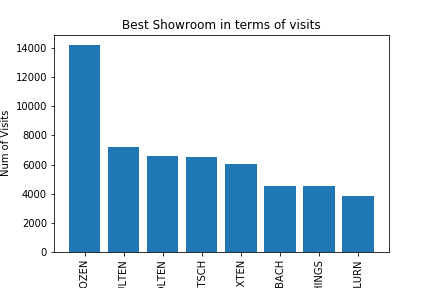
\includegraphics[width=\columnwidth]{../images/best_showroom.png}
        \caption{
                \label{fig:best_showroom}  
                Best running Showroom
        }
\end{figure}

Figure \ref{fig:best_showroom} shows the number of visitors per showroom in decreasing order. It becomes clear that the showroom in Bozen has nearly the double number of visitors as the next smaller showroom.

\begin{figure}[H] 
        \centering
        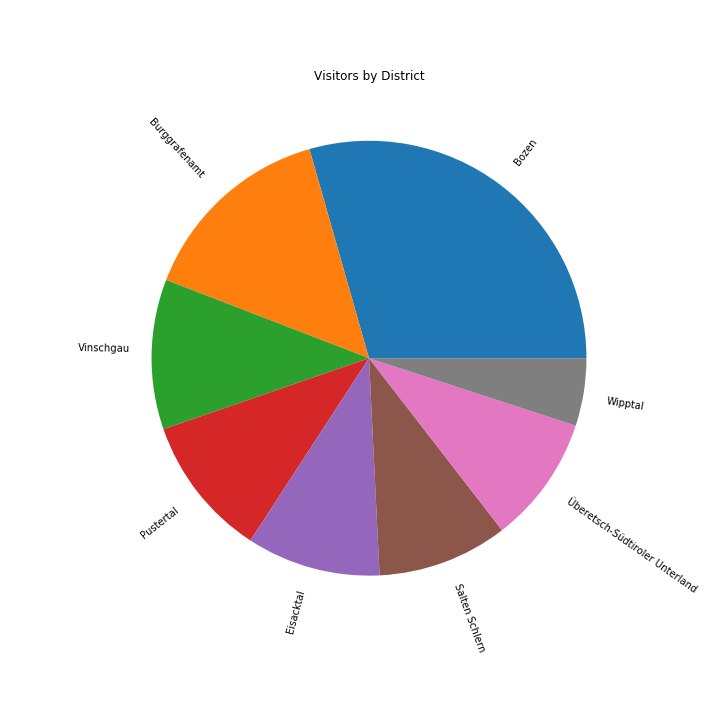
\includegraphics[width=\columnwidth]{../images/district.png}
        \caption{
                \label{fig:district}  
                Visitor District
        }
\end{figure}

Figure \ref{fig:district} shows the number of visitors by their municipality. Again, Bozen is with more than 25\% the biggest chunk.

\begin{figure}[H] 
        \centering
        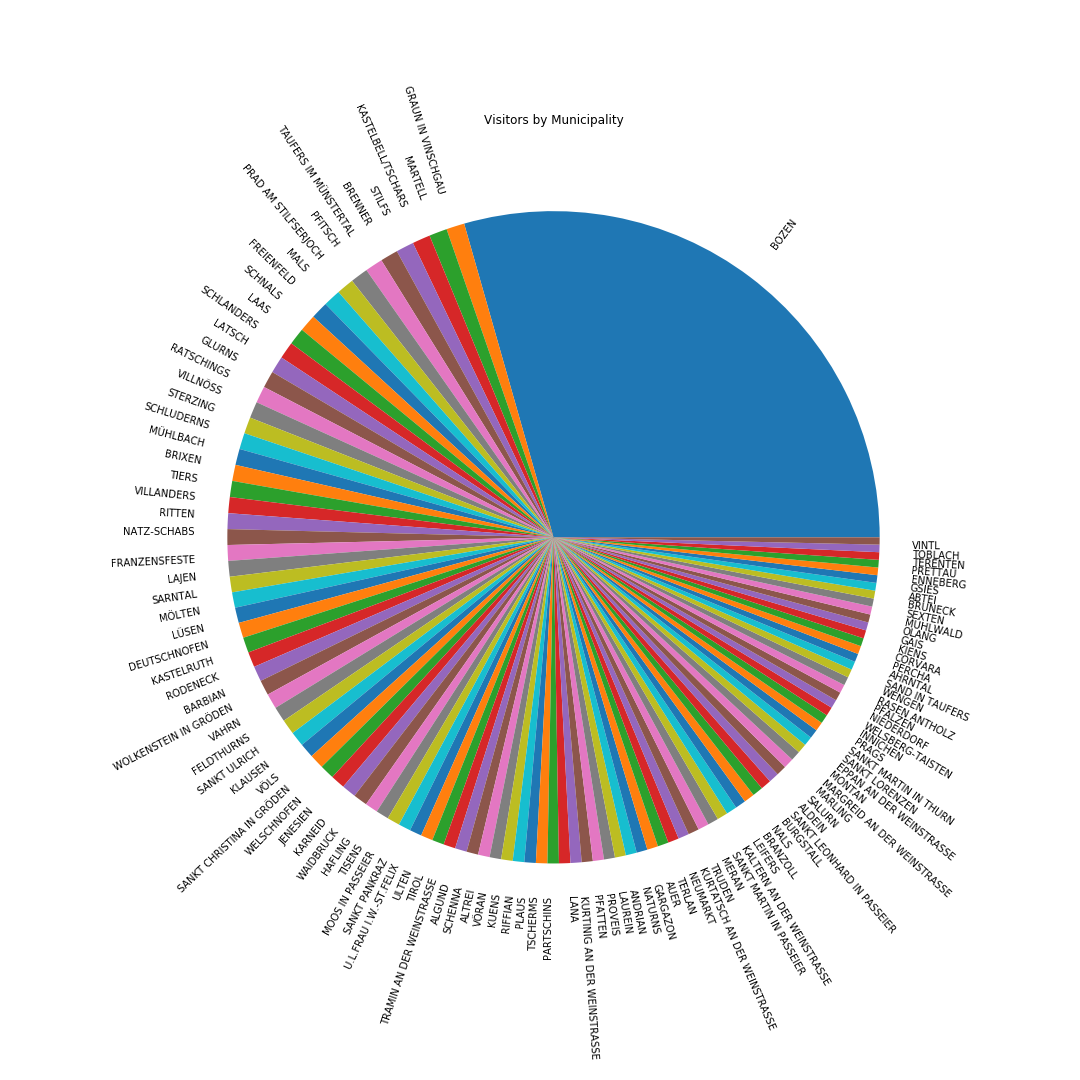
\includegraphics[width=\columnwidth]{../images/municipality.png}
        \caption{
                \label{fig:municipality}  
                Visitor Municipality
        }
\end{figure}

Figure \ref{fig:district} shows the number of visitors per district. Bozen outnumbers all other districts whereas the lowest number of visitors come from Wipptal.

\begin{figure}[H] 
        \centering
        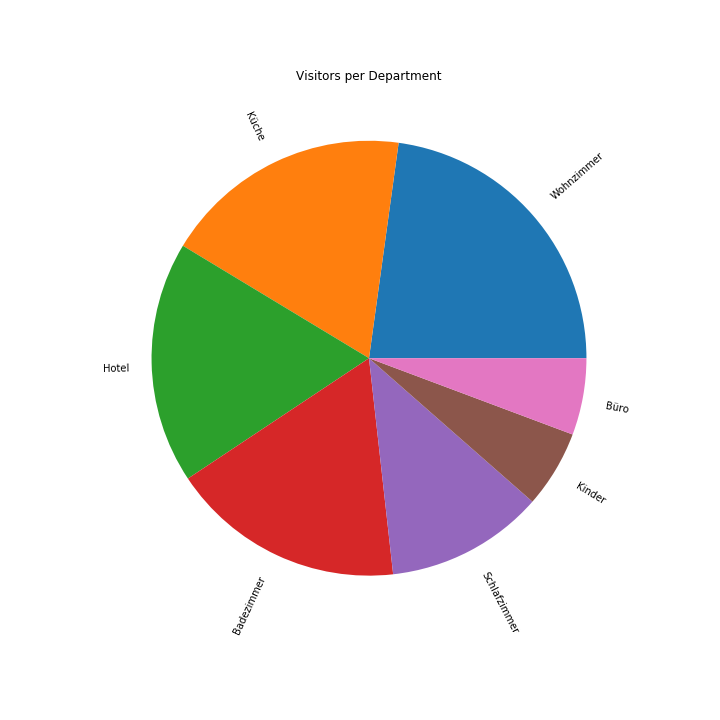
\includegraphics[width=\columnwidth]{../images/department.png}
        \caption{
                \label{fig:department}  
                Visitors per Department
        }
\end{figure}

The next figure \ref{fig:department} visualizes the number of visitors by department. One can see that Living room, Kitchen, Hotel and Bathroom have similar numbers, whereas Children and Office are a lot smaller.

\begin{figure}[H] 
        \centering
        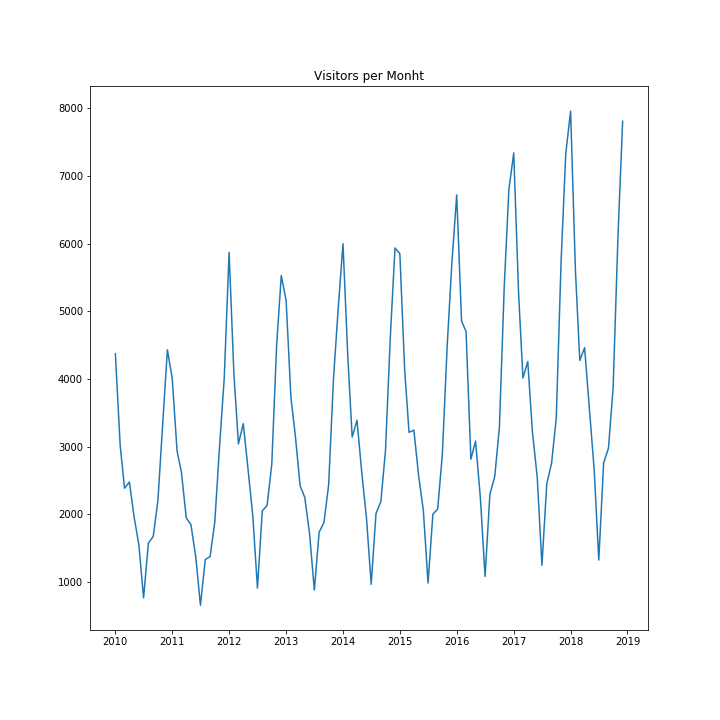
\includegraphics[width=\columnwidth]{../images/month.png}
        \caption{
                \label{fig:month}  
                Visitors per Month
        }
\end{figure}

Figure \ref{fig:month} shows the trend of how many visitors come to all showrooms over time. It becomes evident, that winter is a lot better than summer.

\begin{figure}[H] 
        \centering
        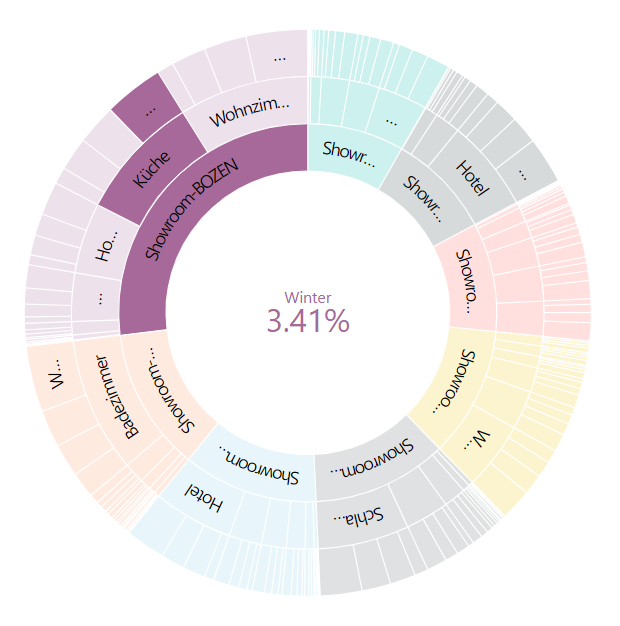
\includegraphics[width=\columnwidth]{../images/sunburst.PNG}
        \caption{
                \label{fig:sunburst}  
                Sunburst Diagram of ROLLUP query
        }
\end{figure}

Figure \ref{fig:sunburst} is a screen shot from a Power-Bi report. The type of the diagram is sunburst. It is interactive and you are able to choose different levels of granularity in order to understand how many visitors you have for example in Bozen in the Kitchen department during the winter season.

\end{document}